\chapter{Introduction}\label{ch:introduction}
This report documents the development of a path-finding robot,
with the purpose of bettering the groups understanding of computation on a microprocessor based platform.

The set goal of the robot was to be able to find the most efficient way
from a given starting point to a given destination on any map.
The idea for this project stems from rescue situations,
where it would be unsafe for a human rescuer to enter the area.

In order to make this feasible within the limits of this project,
we adapted the RoboCup Junior Rescue rules \cite{Robocup}.
Those limitations are mainly about the map and surface,
and have been altered slightly,
to fit the semesters requirements and available time.

\todo{analysis}
\begin{figure}[!ht]
	\centering
	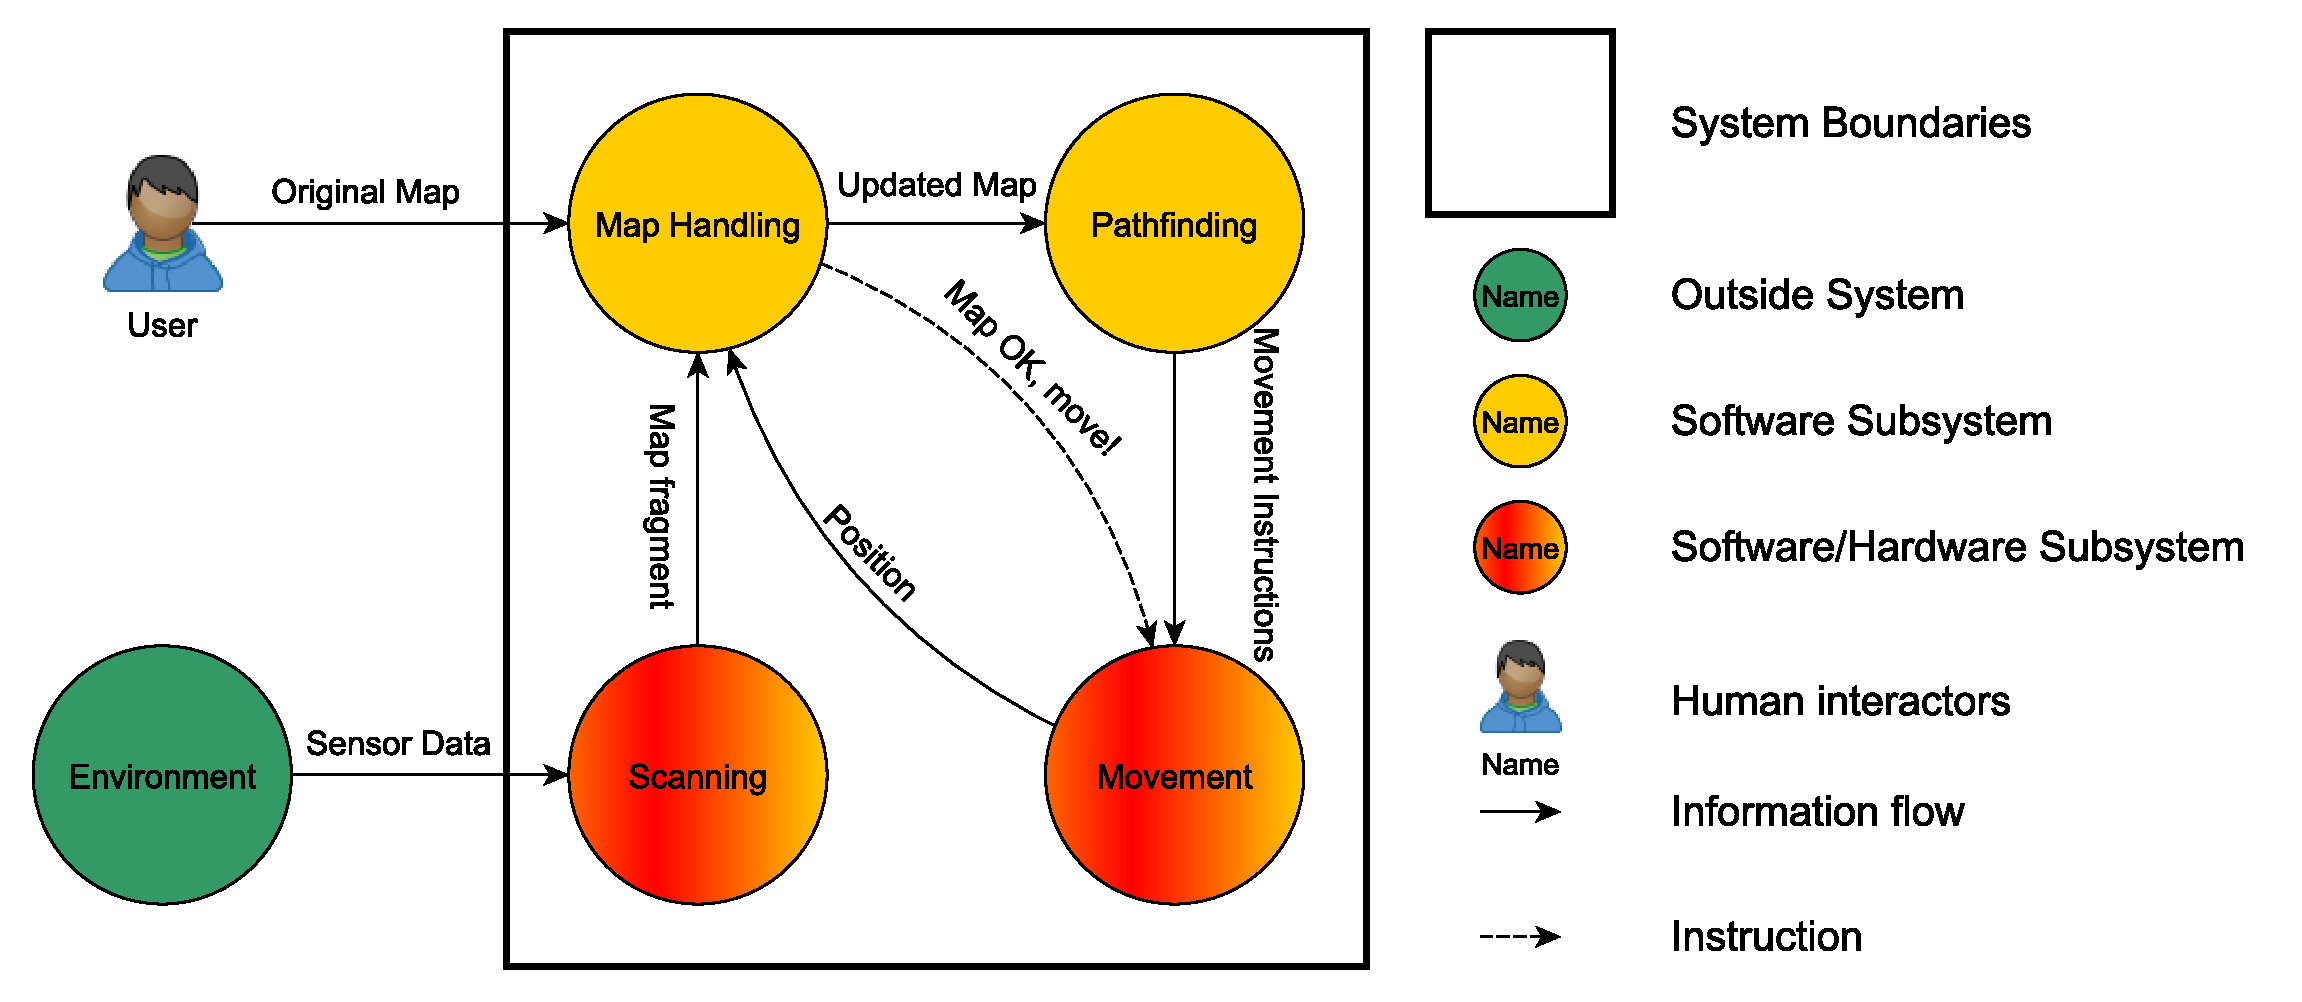
\includegraphics[width=\textwidth]{figures/intro/systemview}
	\caption{Overview over the Robot with Subsystems}
	\label{fig:system} 
\end{figure}
After analysing the problem and our options,
we came to the conclusion,
that a modular system,
as described in Figure \ref{fig:system},
would fit our needs best.

Modularising a system makes simultaneous development of subsystems
and independent testing possible.
Our approach divides the system in four subsystems,
two of which are pure software systems,
the other two a mixture of software and hardware.

We were able to test our software solutions independent from any hardware,
\todo[inline]{something delivery problems}
In the course of our project work,
we encountered some problems with hardware delivery.
Because we modularized our system,
we were still able to work on it without having most of our hardware.

\todo{explain sectioning, based on the modules}


\todo[inline]{this is how far I am with writing the introduction}
\todo[inline]{The next paragraphs may contain some more information, don't know how to put them right now}

In this project we want to talk about path finding algorithms,
with the main focus of building an example implementation on a small scale.

We expect the reader to have a basic understanding of math, programming and simple physics.
But will explain the applied topics.
\todo[inline]{write introduction, should include Problem statement, general idea,}

Autonomous movement can be useful in rescue missions,
where the area is too dangerous to send a human rescuer.
Such environments could be for example:
Burned down/burning houses, buildings struck by natural disaster
or any other building with unknown structural integrity.
